\RequirePackage{ifpdf}
\documentclass[a4paper,11pt]{kth-mag}
\usepackage[T1]{fontenc}
\usepackage{textcomp}
\usepackage{lmodern}
\usepackage[latin1]{inputenc}
\usepackage[swedish,english]{babel}
\usepackage{modifications}
\usepackage{graphicx}
\usepackage{subfigure}
\usepackage{cite}
%\usepackage{url}
\usepackage{hyperref}

\title{Automatic Grading System in Microsoft .NET Framework}

\subtitle{Evaluating the performance of different languages on the Microsoft .NET platform}

\foreigntitle{Automatr\"{a}ttning i Microsoft .NET Framework}

\author{William Lundin Forss\'{e}n}
\date{April 2012}
\blurb{Master's Thesis at NADA\\Supervisor: Alexander Baltatzis\\Examiner: Olle B\"{a}lter}
\trita{TRITA xxx yyyy-nn}


\begin{document}
\frontmatter
\pagestyle{empty}
\removepagenumbers
\maketitle
\selectlanguage{english}


\begin{abstract}

A common challenge for software consulting companies is recruiting the right people. In the software industry, the recruitment process usually involves several steps before a contract is signed; a single job interview is rarely enough. Thus, the interview tends to involve some test to make sure that the person seeking the position is qualified. The testing procedure is usually  part of the interview or conduct at the same occasion. Interviewing applicants who are not qualified for the position might be a waste of time.

This waste can be minimized by only interviewing qualified applicants. In the software industry, qualifications are commonly asserted by letting an applicant solve programming problems. This process can be automated using an Automatic Grader. Such systems already exist on some universities today and are used extensively in various programming courses and also in programming contests.

This thesis evaluates such a system with regard to execution speed and memory consumption. It also explains how such a system can be built and attempts to demonstrate the performance differences between the supported programming languages. The system is unique in the aspect that it is built using only Microsoft .NET Framework while still supporting multiple programming languages. The supported languages are C\#, Java and Python. This support is enabled through the use of a Java byte code to CIL compiler called IKVM. Python is supported through the use of IronPython.

The results showed that C\# and Java performed almost equally in terms of execution speed and memory usage, with Java being slightly behind. As a compensation for Javas slower execution speed a scaling factor was created. The average of this scaling factor was 1.29. Python had greater performance and memory issues than the other two and no scaling factor could be created for this language.

Future work involves implementing additional language support and improving the system with usability in mind.


\end{abstract}


\clearpage

\begin{foreignabstract}{swedish}

En gemensam utmaning för konsultföretag inom mjukvaruutveckling är att rekrytera rätt personer. Rekryteringsprocessen inom mjukvaruindustrin innefattar vanligtvis flera steg innan ett anställningsavtal undertecknas. Enbart en anställningsintervju räcker sällan för att avgöra en sökandes lämplighet. Således tenderar intervjun att involvera någon form av test för att se till att sökanden är kvalificerad. Testproceduren är oftast en del av intervjun eller genomförs vid samma tillfälle. Att intervjua sökande som inte är kvalificerade för positionen i fråga kan vara ett slöseri med tid.

Detta slöseri kan minimeras genom att endast intervjua kvalificerade sökanden. Inom mjukvaruindustrin säkerställs kvalifikationer vanligtvis genom att låta sökanden lösa programmeringsproblem. Denna process kan automatiseras med hjälp av ett s.k.Automaträttningssystem. Sådana system finns redan på flera universitet i dag och används i stor utsträckning i flera programmeringskurser och förekommer även i samband med programmeringstävlingar.

Denna uppsats utvärderar ett sådant system med hänsyn till exekveringshastighet och minneskonsumtion. Den förklarar också hur ett sådant system kan byggas och hur de olika språken presterade. Systemet är unikt i och med att det är byggdes med enbart Microsoft .NET Framework och samtidigt klarar av att stödja flera olika programmeringsspråk. De språk som stöds är C\#, Java och Python. Detta stöd möjliggjordes genom användning av en Java byte-kod till CIL kompilator som kallas IKVM och Python stöds genom användning av IronPython.

Resultaten visar att C\# och Java presterar nästan lika med hänsyn till exekveringshastighet, med Java på andraplats. En skalningsfaktor togs fram som en kompensation för Javas långsammare exekveringstider. Medelvärdet på denna skalningsfaktorn var 1.29. Python verkade ha större prestanda- och minnesproblem än de andra två och ingen skalningsfaktor för detta språk kunde tas fram.

Framtida arbete omfattar stöd för fler programmeringsspråk och förbättra systemet med användbarhet i åtanke.

\end{foreignabstract}


\chapter*{Foreword}

This report is my Master Thesis project which was carried out at Valtech in Stockholm, Sweden. This thesis is part of my last course in the Masters Programme in Computer Science at The Royal Institute of Technology (KTH). The most difficult part of this thesis was finding out what subject to research. Then one day some words from my supervisor Alexander Baltatzis echoed in my head from one of his lectures ``Write code in any language and run it in .NET''. That sentence sparked my interest in finding out whether it was actually possible or not, since most people who write programs on the .NET platform do so using C\# or Visual Basic, you barely ever hear about someone using any other language (even though many others are supported by the .NET platform). 

\chapter*{Glossary}

\begin{center}
	\begin{tabular} { m{3cm} | m{11cm} }
		\hline
		\textbf{Term}	& \textbf{Description} \\ \hline
		CES				& Code Evaluation System, also known as Automatic Grading System, a system for evaluating or grading code. \\ \hline
		CIL				& Common Intermediate Language, the lowest level human-readable programming language in .NET Framework. \\ \hline
		CLI				& Common Language Infrastructure, a specification that describes the runtime environment of Microsoft .NET Framework. \\ \hline
		CLR				& Common Language Runtime, is the virtual machine of Microsoft .NET Framework. \\ \hline
		GUI				& Graphical user interface, an interface that is image oriented rather than text oriented. \\ \hline
		IKVM			& An implementation of the Java for Mono and Microsoft .NET Framework. \\ \hline
		IL				& Intermediate Language, a language of an abstract machine. \\ \hline
		IronPython		& An implementation of the Python programming language targeting the Microsoft .NET Framework and Mono. \\ \hline
		Mono			& An open source project created to enable .NET Framework cross-platform compatability. \\ \hline
		MSIL			& Microsoft Intermediate Language, a synonym for CIL. \\ \hline
	\end{tabular}
\end{center}



\clearpage

\tableofcontents*

\mainmatter
\pagestyle{newchap}

\chapter{Introduction}

\section{Problem Statement}
A common challenge for Valtech and other consulting companies is to recruit the right people. The recruitment process in the IT business often involves several steps and can be time consuming. This is because knowledge and skill can differ significantly from programmer to programmer and a need to interview many people arises (just to find one that is deemed suitable for the job).

Nämn i introduktionen att man syftar att rekrytera folk från högskolan där implementationen av vissa algoritmer är viktigt ur effektivitssynpunkt. Det gäller naturligtvis att även inspektera koden och kolla dess exekveringstid.

The recruitment process usually involves some test to assert the skill of the programmer. A test which usually contains one or several programming problems. The test is sometimes performed on paper (questionnaire) or a white board. Both of these environments are not suitable for programming, hence most programmers tend to do their work on computers with the assistance of a web browser and a suitable IDE.

The testing process is particularly common when it comes to the recruitment of recently graduated university students. On universities, the efficiency of the implementation of certain algorithms are of great importance for the students since they are sometimes graded with this in mind.

These issues present a challenge. The optimal solution would result in less time spent recruiting and at the same time asserting the skills of the programmers before an interview is considered.


\section{Goal}
The main goal was to evaluate a system which could satisfy the demands stated above. Thus, since no such system was present at Valtech, there was a need to build the system and then evaluate it through test cases with performance and memory consumption in mind.

The system would allow users to submit solutions to common programming problems and then have their code evaluated. Their code would have to have a limit on execution time since a ``good'' programmer should be able to solve problems efficiently, particularly common university style algorithms such as sorting. The results of the evaluation would be used to estimate how much time the different programming languages would need in order to solve problems as all of these languages would be run in the Microsoft .NET Platform and some are expected to perform better than others.


\section{About Valtech}
Valtech is an independent, global IT-consulting company with offices in Europe, United States and Asia. The company was founded 1993 in France and has over 1600 employees worldwide. The Swedish division is primarily oriented towards web solutions. Some of Valtech’s most well-known award winning projects includes the websites 1177.se, Antagning.se and Riksbank.se.

All work concerning this thesis was carried out at Valtech in Stockholm, Sweden.









\chapter{Background}

\textit{This chapter gives a short presentation of what automatic grading is, some history and how the systems that are in use today are built.}

\section{What is automatic code evaluation?}
Automatic code evaluation, or automatic grading, is a computer system that has the ability to judge code. The process starts with the user being given a programming task or problem to solve. The user then attemps to solve this problem by writing some code which he or she then sends to the automatic code evaluation system. The system compiles the code (if needed) and then runs it. The output generated is then compared with the correct output for that particular problem. If the output matches, the system returns a status message indicating a successful submission (e.g. ``Accepted'') or if the output doesn't match a different message is returned, indicating that something went wrong (e.g. ``Wrong answer''). 

There are some variations to the process above, sometimes more verbose feedback than ``Wrong answer'' is used, often indicating exactly which test went wrong and why \cite{Gradebot}. This is usually done in order for university students to learn more about how to code by debugging/fixing their own code.

Having an automatic grading system results in several benefits \cite{Suleman}. There is no longer a need for humans correcting code in detail (a very time consuming process) since the system acts as a ``judge''. Using this judge also gives greater consistency while evaluating code since all submissions are judged equally. The system can provide instantaneous feedback, making the waiting time considerably shorter, this is particularly true for universities where students no longer have to wait for a teacher or an assistant to grade their homework. Submissions to this system are saved using a database, providing whoever administrates the system a way to trace all interactions with it.


\section{History}
The concept of automatic grading is not new. The earliest known system was built in 1960 by Hollingsworth \cite{Hollingsworth}. This system used punch cards to write programs. The results from using this student-system approach rather than the traditional student-teacher was that it cut costs considerably for the staff since the time they needed to grade the students work was sverely reduced. The students themselves also spent less time on each task, since they were able to have their work graded immidiately instead of waiting for a teacher to do it. This system also made it possible to considerably increase the number of students taking the course. It did, however, have some shortcomings. For instance, a student's program could modify the grader program, making cheating possible. 

An article from 2005 \cite{GenerationReview} describes three generations of automatic graders. The first generation systems were those regarded as being built and/or used in the 1960's and 1970's. Unsurprisingly, they used code that were close to pure machine code. In order to make them work, it was sometimes necessary to modify both the compiler and the operating system. 

The second generation systems (1980-2000) introduced script-based tools. These involved various verification schemes and also asserted that the code was written in a certain way/style (decided by the teacher). Typically these graders involved command-line GUI:s. Languages like C and Java were used extensively.

The third generation (2000-) differ from the second generation systems primarily in two ways. One is that they mostly use web based GUI:s. The other is that they often included a plagiarism detection system, since students sometimes shared code amongst each other. There were some minor issues among these detection systems \cite{GenerationReview} \cite{Gradebot} . If the programming task was too simple or if a lecturer had been excessively thorough when describing the homework, the submissions would tend to be very much alike and thus picked up by the plagiarism detection system. Sometimes this made it difficult to distinguish between real plagiarism and the false positives. 

\section{Todays systems} \label{sec:todays_systems}
Todays modern systems, such as those in \cite{Gradebot} \cite{Suleman} \cite{GenerationReview}  \cite{Kattis} \cite{Amelung} (considered to be third generation systems), commonly contain a web based front-end together with a general back-end whos main purpose is to save submissions to the database and to send the submitted code (pipeline) to the other language specific back-ends (one for each language) while preserving system security through sandboxing. The database can be used to inspect specific submissions. The modern systems mainly differ in their support of different programming languages. 


\chapter{Method}
This chapter explains how the system was implemented. It contains details about the work-flow, the GUI, how multiple languages are supported, how the security works and some of the difficulties and limitations encountered.

\section{System Description}
The system was named CELINE, an abbreviation that comes from the descriptive phrase ``\textbf{C}ode \textbf{E}va\textbf{L}uation \textbf{I}n .\textbf{NE}t''.

\begin{figure}[h]
	\centering
	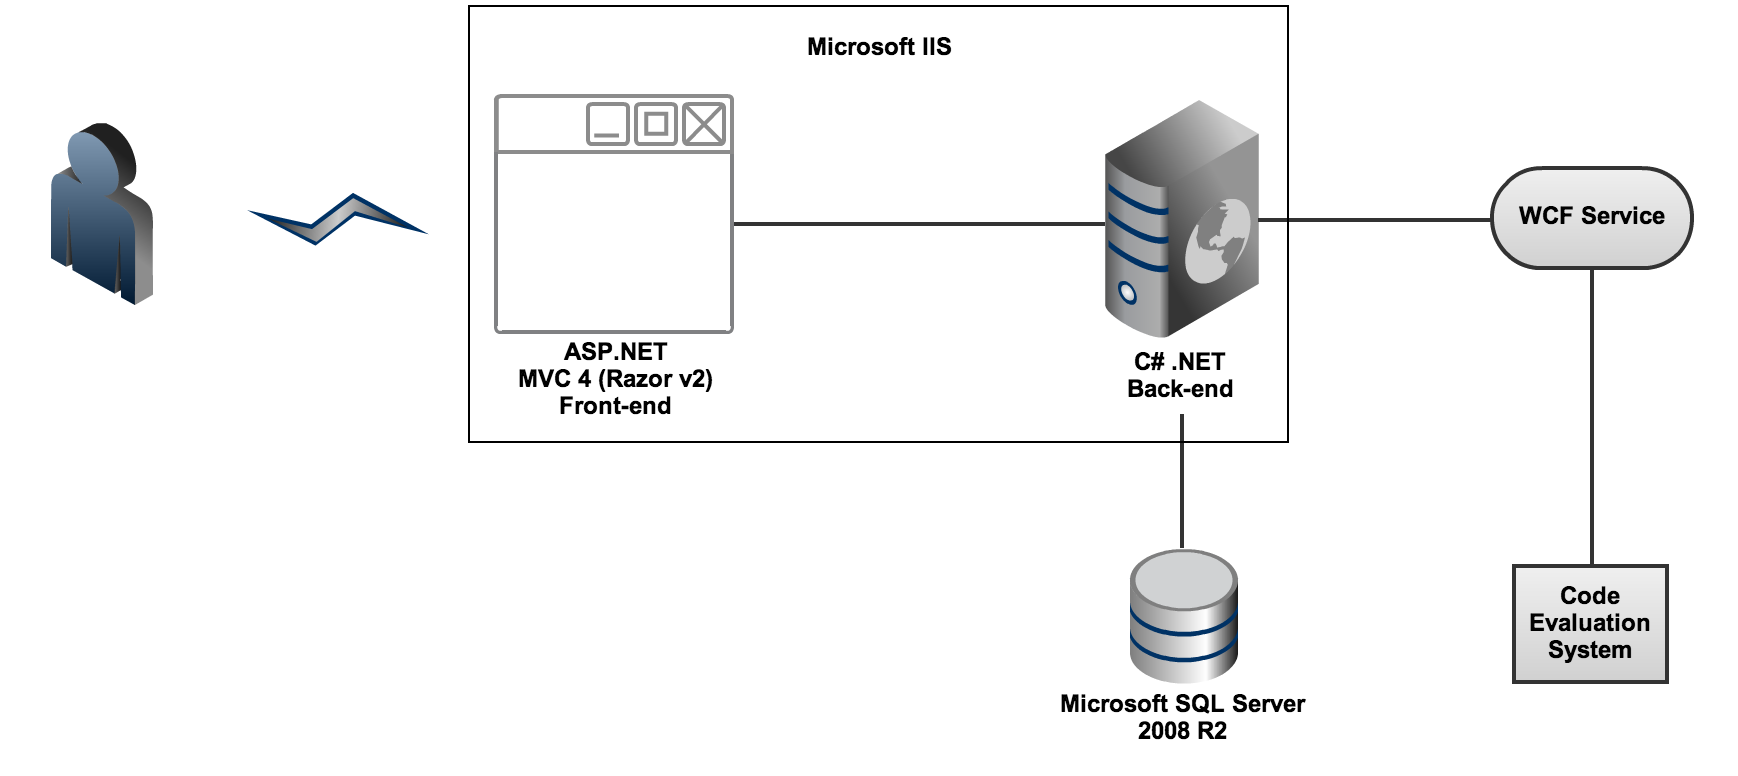
\includegraphics[width=0.9\linewidth]{chapters/media/overview.png}
	\caption{Overview of CELINE.}
	\label{fig:SystemOverview}
\end{figure}

Figure \ref{fig:SystemOverview} describes an overview of the system. The system uses a web based GUI for listing problems and submitting solutions to them. Going through this figure from left to right we can see that a user connects to the website through a web based GUI, which is built using a combination of ASP.NET MVC4 (Razor v2) technology and JavaScript. The system uses Microsoft IIS to enable this web support, which is the standard web server software used in .NET. When the user submits code to solve a problem, that submission is saved to a database which is a Microsoft SQL Server 2008 R2 database. The submission is then forwarded to a WCF Service which in turn creates a new instance of the automatic grading system (built using C\#) using the submission as input. The automatic grader compiles the source if needed and runs the code. It then returns a status code generated from the submission, this is described in section \ref{subsec:status_codes}.


\subsection{The Web GUI and workflow}
The GUI is built using the ASP.NET MVC4 template. This saved both time and effort while still giving the website an easy to understand simplistic style.

\begin{figure}[h]
	\centering
	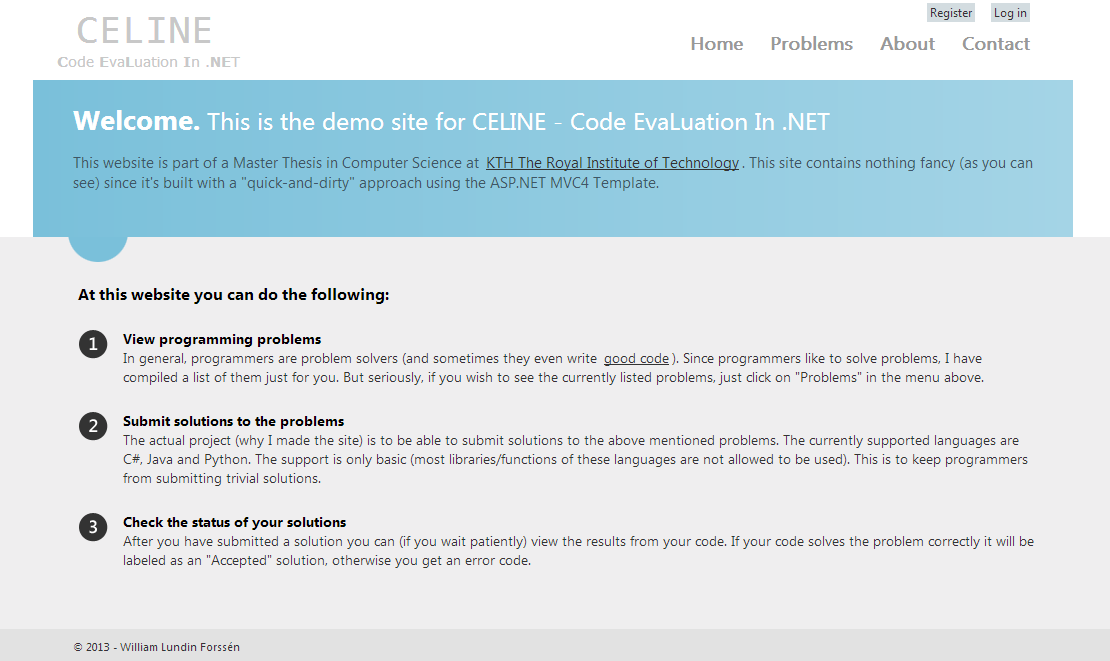
\includegraphics[width=1.0\textwidth]{chapters/media/celine_startpage.png}
	\caption{The start page of CELINE.}
	\label{fig:celine_startpage}
\end{figure}

In Figure \ref{fig:celine_startpage}, we see the start page. This is the page where applicants start their workflow. The middle area contains some informative text; the top right contains the site menu, the register and login buttons.

From the start page an applicant may click on the ``Problems'' text in the top-right corner which sends them to a page containing a list of problems, see Figure \ref{fig:celine_list_problems}.

\begin{figure}[h]
	\centering
	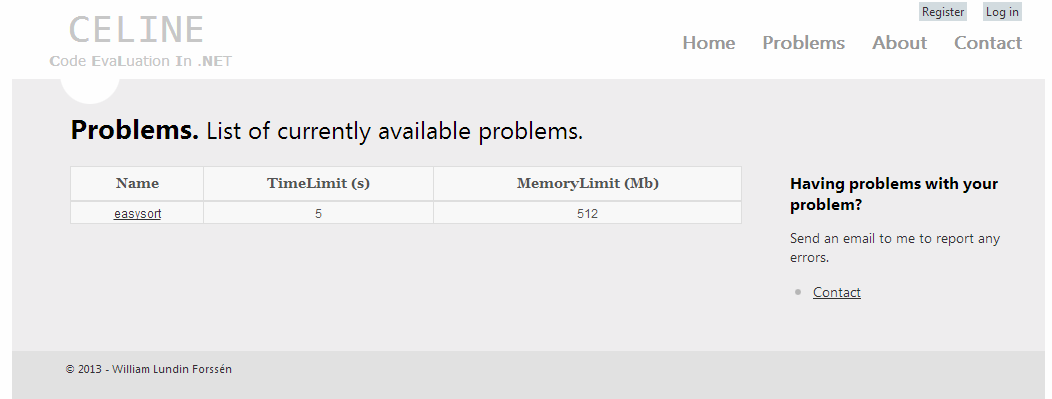
\includegraphics[width=1.0\textwidth]{chapters/media/celine_listproblemsCut.png}
	\caption{Listing of available problems page. This page is shown when a user clicks on the ``Problems'' text in the top-right. One of the available problems is called ``easysort''. }
	\label{fig:celine_list_problems}
\end{figure}

Should the applicant find a problem they want to solve, they simply click on that problem in the list to arrive at an information page containing that specific problem, see Figure \ref{fig:celine_easysort}. If the applicant wants to solve this particular problem they may click on the ``Submit solution'' button (visible on the right side).

\begin{figure}[h]
	\centering
	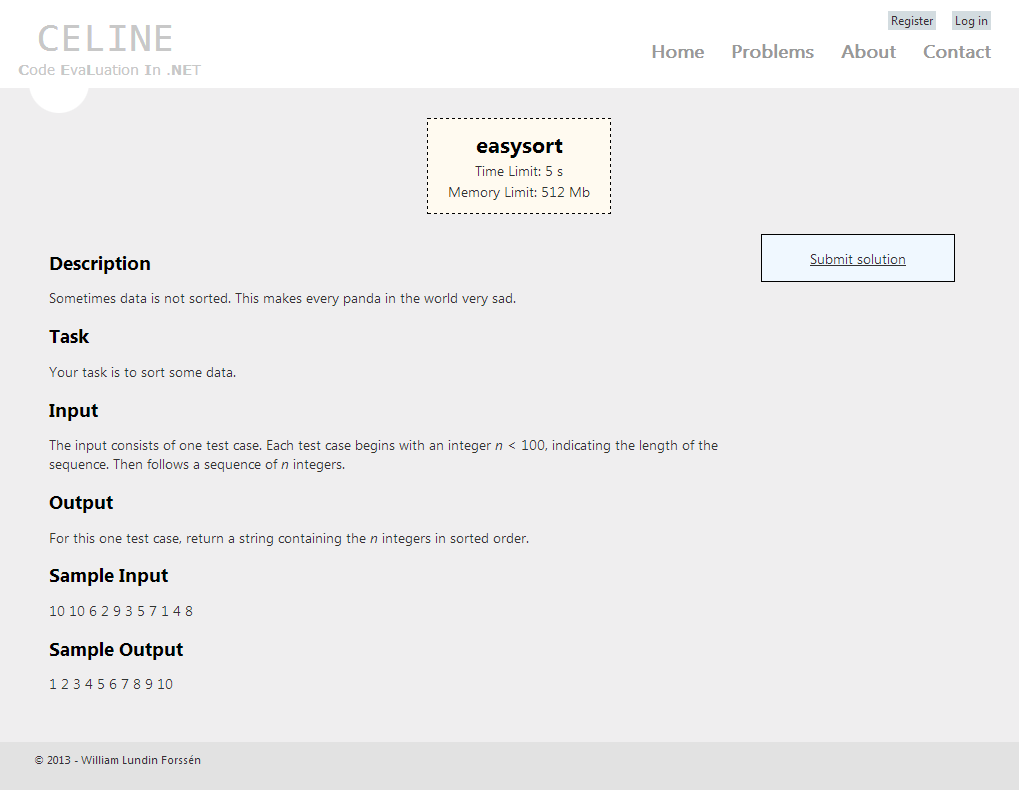
\includegraphics[width=1.0\textwidth]{chapters/media/celine_easysort.png}
	\caption{Problem information page. This is where applicants can read about the problem statement and get information regarding what to expect as input and what the system expects their solution to output.}
	\label{fig:celine_easysort}
\end{figure}

In Figure \ref{fig:celine_submit}, we see the submission form on the left side, this page contains some useful information on the right side concerning language-specific signatures. These signatures specify the point of entry for the application (where the execution of the code starts). Users are free to name this method to anything they see fit, the only limitation is that it takes a string as input and returns a string as output. This is discussed in further detail in section \ref{subsec:status_codes}.

\begin{figure}[h]
	\centering
	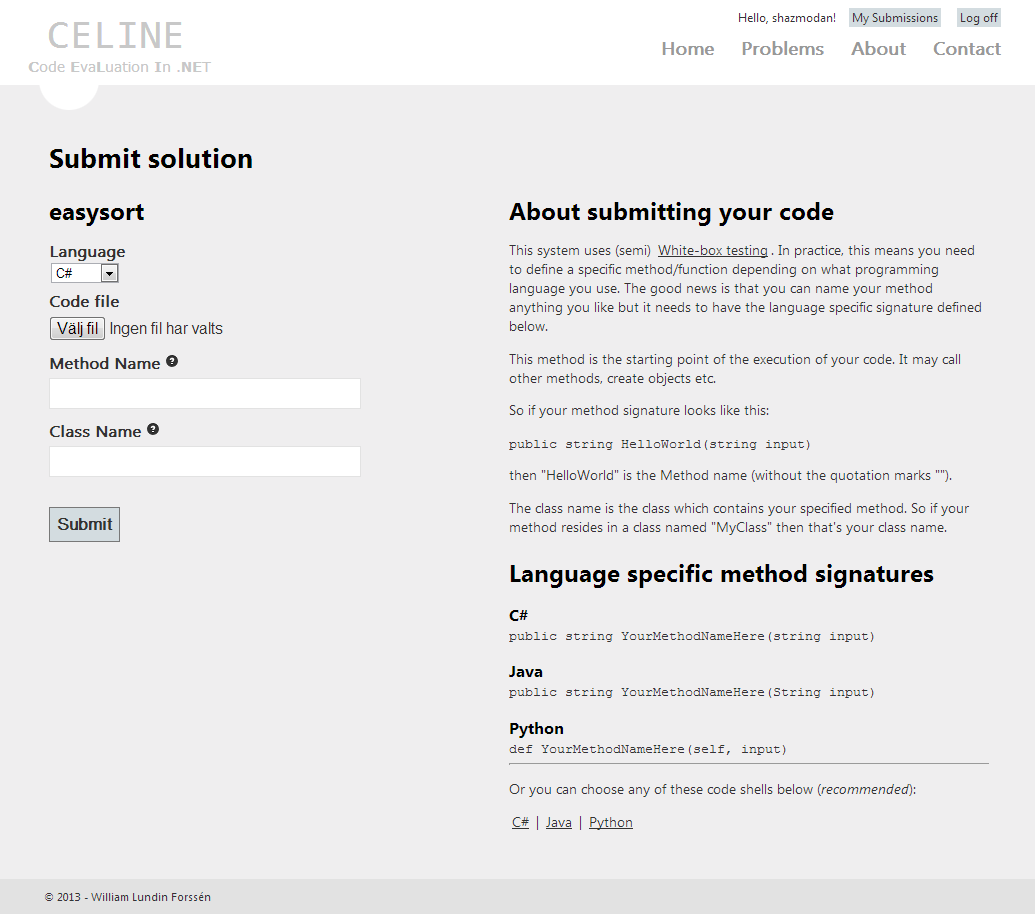
\includegraphics[width=1.0\textwidth]{chapters/media/celine_submit.png}
	\caption{Code submission page. This page provides the user with details regarding submitting a solution to a problem. The system requires that a specific programming language to be selected from the drop down list at the top, a main class name and a specified method signature (acting as the application's entry point).}
	\label{fig:celine_submit}
\end{figure}

When the applicant has submitted their solution, they are sent to a page where they can see all of their submissions, see Figure \ref{fig:celine_submissions}.

\begin{figure}[h]
	\centering
	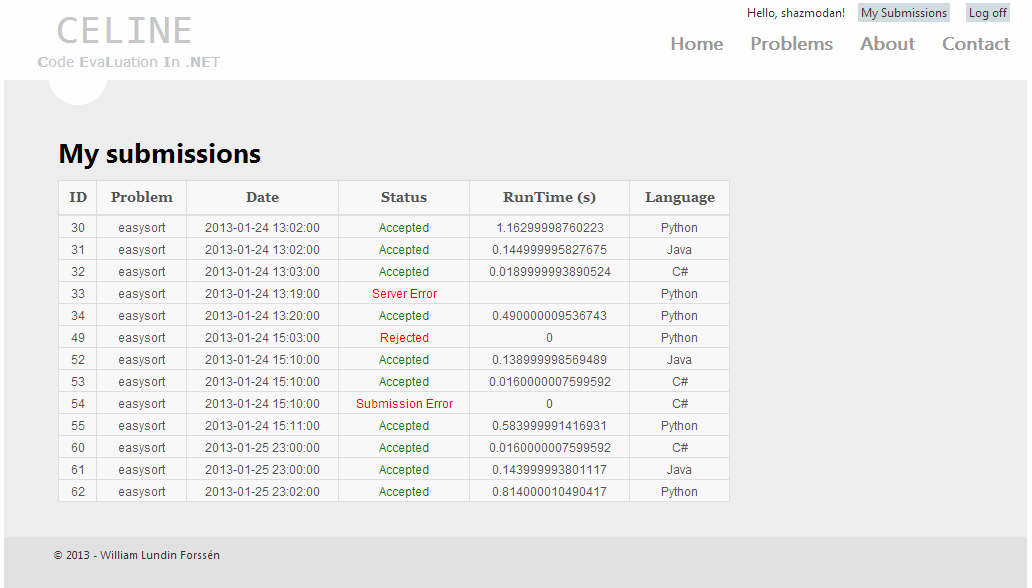
\includegraphics[width=1.0\textwidth]{chapters/media/celine_submissionsCut.png}
	\caption{All submissions page. This page displays a list of all submissions that an applicant has made. Each item in the list contains a unique id, the name of the problem, the date of when the submission was sent, the status code which indicates if the output was accepted or not, the time it took for the output to be produced and the language that was used.}
	\label{fig:celine_submissions}
\end{figure}


\subsection{The Automatic Grading System}
When a user has submitted his or her code, it eventually reaches the AGS. Figure \ref{fig:flowchart} describes the flow of the most common paths for a submission through the system.

\begin{figure}[h]
	\centering
	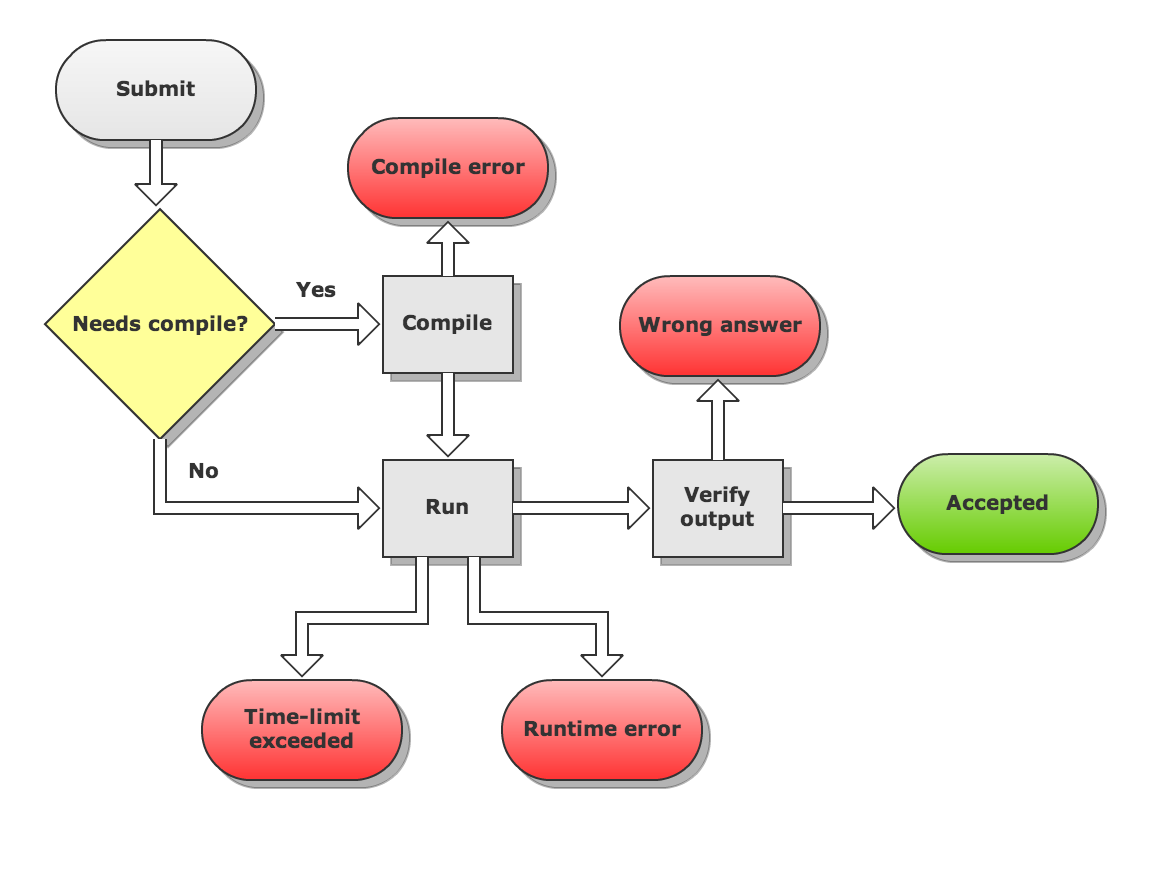
\includegraphics[width=0.8\linewidth]{chapters/media/flowchart.png}
	\caption{Common paths of problem flow in the AGS.}
	\label{fig:flowchart}
\end{figure}

Depending on the programming language, a compiler is chosen. The code is then compiled into an assembly file and loaded into a separate and secure Application Domain (AppDomain, see section \ref{subsec:security}). The AGS then invokes the user specified method with a string containing the test data. The AGS waits for the code to complete or for the problem to timeout. The timeout is problem specific and decided when the problem is created. It then compares the string returned by this method with another string containing what should be the correct output. If the strings match, the submission is regarded as being a success; otherwise it is regarded as a failure. The AGS then returns the appropriate status code.


\subsection{System-User Feedback} \label{subsec:status_codes}
The system gives feedback to the user in the form of a status code, one for each submission. The status code is a simplistic message that indicates whether the submission was successful or not. This system attempts to be more verbose on errors than other modern systems (described in section \ref{sec:todays_systems}). It uses grey-box testing, which is more prone to submission related errors, than black-box testing (commonly used in today's AGS:s). The concepts of white- and black-box testing are described more thoroughly in section \ref{subsec:whitebox_blackbox}. The following list contains the possible status codes:

\begin{itemize}
	\item Accepted - The code has compiled, run and gave the correct answer.
	\item Wrong Answer - The code has compiled and run but gave the wrong answer.
	\item Server Assembly Error - The AGS failed to build an assembly from the code file, thus making the code unable to run.
	\item Submission Error - The code tries to reference a code library that is not available/allowed.
	\item Illegal Operation - Occurs if the AGS detects a forbidden system call (e.g. accessing files, using the network etc...).
	\item Class or Function Error - Occurs if the class or method name does not correspond to the name provided by the user, thus resulting in the AGS being unable to invoke it.
	\item Time Limit Exceeded - The code ran longer than the time-limit for this problem allowed. This could be an indication that the code needs to be improved (performance wise). The time limit is decided by the admin who created the problem.
	\item Rejected - This is a general error which indicates that the AGS has been unable to determine why the submission failed.
	\item Server Error - This indicates that the AGS instance has crashed.
\end{itemize}

The status messages ``Server Assembly Error'', ``Submission Error'', ``Illegal operation'' and ``Class or Function Error'' are all related to incorrect formatting of the code by the user. These might be less verbose than one would like (e.g. each submission could have returned exactly where in the code the error occurred). Any more verbose feedback would have required an expansion of the scope of this thesis.



\section{Supported languages}

\subsection{C\#}
The support for C\# was implemented with the use of the Microsoft CSharp library (ref http://msdn.microsoft.com/en-us/library/microsoft.csharp.csharpcodeprovider.aspx) and the System CodeDom Compiler library (ref http://msdn.microsoft.com/en-us/library/system.codedom.compiler.icodecompiler.aspx).

\subsection{Java}
The Java support comes from using javac (ref http://www.oracle.com/technetwork/java/javase/tech/javac-137034.html), the standard Java compiler that comes with the Java Development Kit (JDK) (ref http://www.oracle.com/technetwork/java/javase/overview/index.html). Javac compiles Java code to bytecode. This bytecode is then converted to CIL using ikvmc (ref http://sourceforge.net/apps/mediawiki/ikvm/index.php?title=Ikvmc), a tool that is part of IKVM.NET (an implementation of Java for Mono and the Microsoft .NET Framework) (ref http://www.ikvm.net/). 

\subsection{Python}
Python is supported through the use of IronPython (ref http://ironpython.net/). IronPython provides a library which contains a ScriptEngine from which python code can run without the need for compiling. Some issues encountered with the IronPython implementation are discussed in section ???. FIXME 

\section{Difficulties and limitations}

\subsection{Security}

- AppDomains


- Reason for WCF Service


The WCF Service is used to avoid the evaluation system crashing due to stack overflow exceptions which are not possible to try-catch in C\# since version 2.0 (referens  till msdn stackoverflowexception) (workarounds exist but they are discouraged). derrrpp


\subsection{IronPython limitations}

- IronPython limitation
- Python ScriptEngine thing

\subsection{White- and black-box testing}

- White-box testing and black-box testing






\chapter{Testing Methodology}

\section{Aspects to tests}

\subsection{Execution speed}

\subsection{Memory usage}

\section{The chosen tests}
The tests are a mixture of general functionality and two specific algorithms. This section assumes that the reader is familiar with the Big O notation.

\subsection{Language overhead}
Each programming language has an overhead startup cost. This is measured by submitting code which does the minimum given this context. In Figure \ref{fig:language_overhead} a minimum code block for the C\# programming language is demonstrated.

\begin{figure}[h]
	\lstset{style=sharpc}
	\begin{lstlisting}
	public class OverheadTest{
		public string SimpleReturn(string input){
			return "";
		}
		public static void Main(){}
	}
	\end{lstlisting}
	\caption{C\# code for language overhead testing.}
	\label{fig:language_overhead}
\end{figure}

This code will recieve an empty string as input, and return an empty string. Measuring the overhead makes it possible to compensate for a language which has a slower execution time. For example, it would be unfair to restrict Python code to the same time-limit as C\# code, since Python has a considerably longer startup time than the native .NET language C\#. 

\subsection{Common Operators}
The common operators are addition (+), subtraction (-), multiplication (*), division (/) and modulo (\%). This test will measure how the language performs doing the simplest operations, giving an indication of its general performance. Figure \ref{fig:addition_test} shows the code used for the addition test in Python.

\begin{figure}[h]
	\lstset{style=sharpc}
	\begin{lstlisting}[language=python]
	class AdditionTest:
	    def AddNumbers(self, input):
	        input = input.split(" ")
	        sum = 0
	        for x in range(0, len(input)):
	            sum += int(input[x])
	        return str(sum)
	\end{lstlisting}
	\caption{Python code for testing the addition operation.}
	\label{fig:addition_test}
\end{figure}

This code takes a string containing numbers as input, divides it into an array of numbers, sums these numbers and returns this sum.

\subsection{Insertion Sort}
Insertion Sort is a comparison based sorting algorithm useful for sorting small inputs. The algorithm can be expressed using code, but this doesn't illustrate it very well for people not already familiar with it, so instead I will explain it using playing cards (using a common 52 card deck):

\begin{itemize}
\item Start with an empty left hand and imagine yourself seeing a bunch of cards on a table.
\item Pick a card from the table one at a time from left to right.
\item Insert this card into the correct position in your left hand.
\item The correct position is determined by comparing this card to each other card in your hand from right to left.
\item The cards in your left hand are always sorted before each new card is picked.
\end{itemize} 

The algorithm has a runtime of $O(n^2)$ but can still outperform more advanced algorithms such as Merge Sort (described in section \ref{subsec:merge_sort}) because Merge sort has an extra overhead from its recursive function calls and also uses more memory, but this is only true for small inputs (what ``small'' is varies from system to system) \cite{Insertionsort}.

Insertion Sort is a suitable algorithm for testing performance between different languages since its implementation is very simple, straightforward and similar in these languages.


\subsection{Merge Sort} \label{subsec:merge_sort}
Merge Sort is a divide and conquer, comparison based sorting algorithm. It's stable in the sense that it preserves the input order of equal elements in the output. The algorithm goes as follows (once again using the common 52 card deck):

\begin{itemize}
\item Imagine yourself seeing a full deck of cards in a line on a table.
\item Divide the cards into two equally sized piles. There should now be 26 cards on your left side and 26 cards on your right side.
\item Keep dividing these piles in half until you only have piles with one card in them. 
\item Now merge these one card piles together so that you end up with a pile that contains 2 cards that are sorted from left to right (in ascending order).
\item Keep merging all piles together until you end up with one pile containing all of the cards (52) in sorted order.

\end{itemize} 

Figure \ref{fig:mergesort} illustrates this process using eight cards.

\begin{figure}[h]
	\centering
	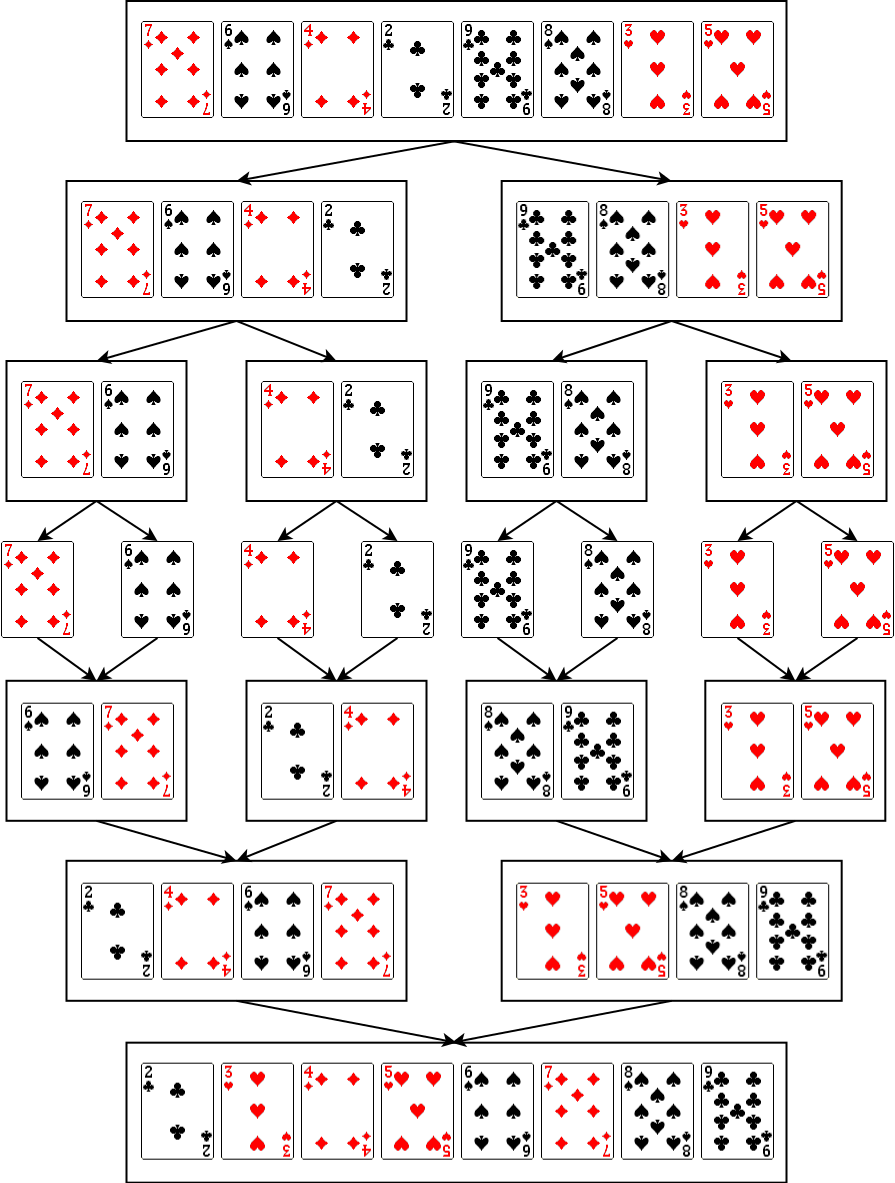
\includegraphics[width=0.9\linewidth]{chapters/media/mergesort4.png}
	\caption{Illustration of the Merge Sort algorithm using eight cards. The cards are subsequently divided up and then merged back together in sorted order.}
	\label{fig:mergesort}
\end{figure}

There are several sorting algorithms that have a worst time complexity of $O(n * log(n))$, Merge Sort was chosen because it has an auxiliary worst space complexity of $O(n)$, thus using more memory than other similar algorithms (e.g. Heap Sort) \cite{Mergesort}. This helps in illustrating how different programming languages differ in memory consumption.







\chapter{Testing Results} \label{chap:results}
\textit{This chapter describes the system specifications of the two computers that were used during testing; how to tests were carried out and present the results of the tests.}


\section{Testing Systems Specifications} \label{sec:system_specs}
The tests were conducted on two computers. The system specifications can be seen in Table \ref{table:system_specs}. The MacBook Pro runs Windows 7 with the help of Parallels Desktop 8. 

\begin{table}[h]
	\begin{center}
		\begin{tabular} { m{4cm} | m{4cm}  | m{5cm} }
			\hline
			\textbf{} & \textbf{MacBook Pro} & 
			\textbf{Windows 8 Desktop}  \\ \hline

			\textbf{Operating System}		& OSX 10.8.2 
											& Windows 8 Pro 64-bit v6.2 \\ \hline

			\textbf{Processor}				& 2.6 GHz Intel Core i7 
											& 2.4 GHz Intel Core2Quad  \\ \hline

			\textbf{Memory}					& 16 GB 1600 MHz DDR3
											& 4GB 400 MHz DDR3 \\ \hline

			\textbf{Parallels Memory}		& 8 GB dedicated memory 
											& --- \\ \hline

			\textbf{Parallels \# CPU:s} 	& 4 dedicated cores
											& --- \\ \hline

			\textbf{Parallels OS} 			& Windows 7 64-bit v6.1
											& --- \\ \hline
		\end{tabular}
	\end{center}
	\caption{System specifications for the computers used.}
	\label{table:system_specs}
\end{table}
It may appear strange that Parallels have four dedicated cores when the Intel Core i7 processor only contains 4 cores, but this is made possible due to the use of virtual cores (8 in total).





\section{Testing Procedure}
All tests presented in this chapter were run on both computers. The ratios on the Windows 8 computer were close to the OSX computer running Parallels and Bootcamp. The small differences in the results between the two machines are likely due to pure variance. The test results should be viewed in relative terms and not in absolute terms.

While the best time is the only time presented in this chapter, the mean-time was also recorded to make sure that the best time was not just a one-time fluke (which could have depended on unknown factors).

Every test was run 100 times on each computer in order to reduce variance. All results were adjusted according to the overhead for each language (see section \ref{subsec:language_overhead}). The input for each test varies from 10'000 elements up to 10 million elements. The elements are randomly generated positive integers.

All tests in the Java and .NET environments were run with disabled debug flags to optimize performance.

All tests results are collected after a warm up of 100 runs (see Section \ref{sec:jit}).


\section{Results}
In this section, the results are presented in table and chart forms. Note that on some charts the vertical axis is base 10 logarithmic. The implementation of all the algorithms for all languages can be found in Appendix blablabla FIXME.


\subsection{Language Overhead} \label{subsec:language_overhead}

\begin{table}[h]
	\begin{center}
		\begin{tabular} { >{\centering\arraybackslash}m{3cm} | >{\centering\arraybackslash}m{2cm} | >{\centering\arraybackslash}m{2cm} }
			\hline
			\textbf{Language}	& \textbf{Time} & \textbf{Ratio} \\ \hline
			C\#					& 0.014s 		& 1:1 \\ \hline
			Java				& 0.038s 		& 1:2.7 \\ \hline
			Python				& 1.006s 		& 1:71.9 \\  \hline		
		\end{tabular}
	\end{center}
	\caption{The overhead startup cost for each language.}
	\label{table:language_overhead}
\end{table}

As can be seen in Table \ref{table:language_overhead} Python has a greater overhead cost than the other two.

\section{Common operators}

\subsection{Insertion sort}

\begin{table}[h]
	\begin{center}
		\begin{tabular} { >{\centering\arraybackslash}m{3cm} | >{\centering\arraybackslash}m{2cm} | >{\centering\arraybackslash}m{2cm} }
			\hline
			\textbf{Language}	& \textbf{Time} & \textbf{Ratio} \\ \hline
			C\#					& 0.078s 		& 1:1 \\ \hline
			Java				& 0.131s 		& 1:1.7 \\ \hline
			Python				& 12.525s 		& 1:160 \\  \hline		
		\end{tabular}
	\end{center}
	\caption{Results of the insertion sort test.}
	\label{table:insertion_sort}
\end{table}

Table \ref{table:insertion_sort} illustrates the time it takes for each language to sort 10'000 positive integers in random order. 

\subsection{Merge Sort}

\begin{figure}[h]
	\centering
	\mbox{
		\subfigure[Test results from Merge Sort when run in .NET.]{
			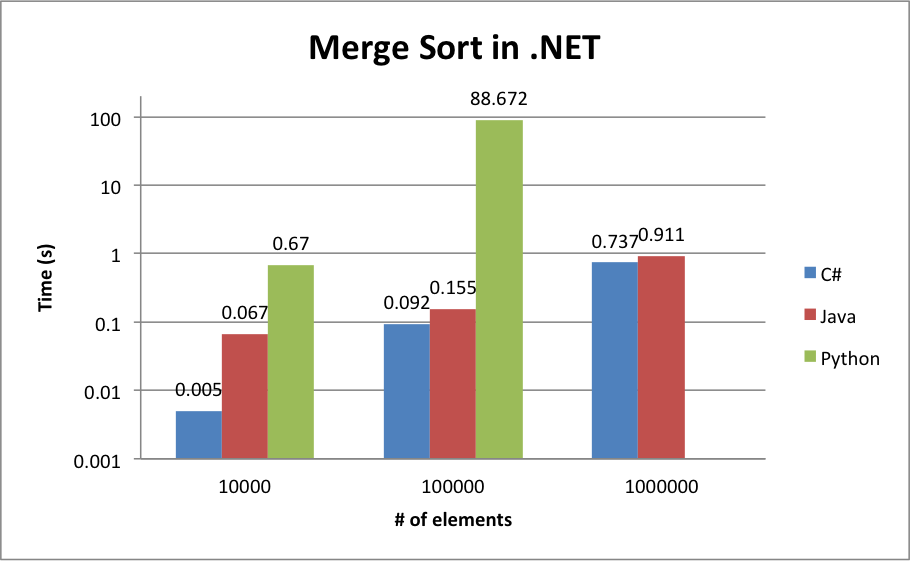
\includegraphics[width=0.48\textwidth]{chapters/media/merge_sort_all_net.png}
			\label{fig:merge_sort_all_net}
		}
		\subfigure[Test results from Merge Sort when run in native environments.]{
			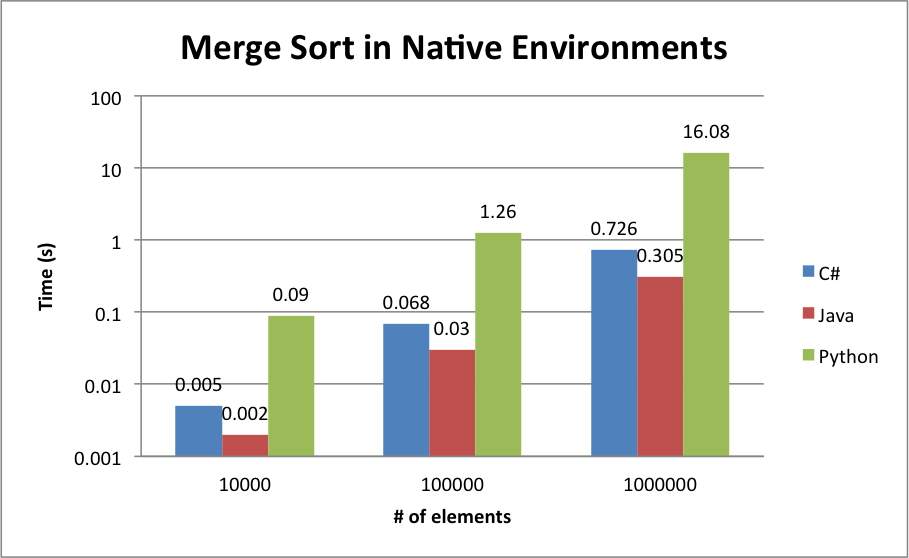
\includegraphics[width=0.48\textwidth]{chapters/media/merge_sort_all_native.png}
			\label{fig:merge_sort_all_native}
		}
	}
	\caption{Comparison of running Merge Sort in .NET to the left and each language native environment to the right.}
	\label{fig:merge_sort_net_native}
\end{figure}


Running code in its native environment provides a big increase in performance for Merge Sort as well, see Figure \ref{fig:merge_sort_net_native}. This gap seemed to get narrower when increasing the amount of numbers to be sorted.

C\# still outperforms Java when run in the .NET environment. But the gap between them seemed to narrow the more elements were added (see Figure \ref{fig:merge_sort_all_net}). 

\begin{figure}[h]
	\centering
	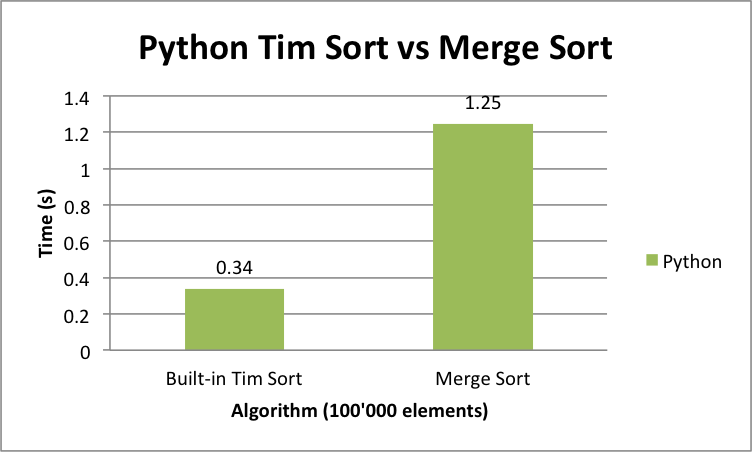
\includegraphics[width=0.6\textwidth]{chapters/media/tim_sort.png}
	\caption{Python built-in function Tim Sort vs Merge Sort.}
	\label{fig:tim_sort}
\end{figure}

Figure \ref{fig:tim_sort} illustrates the performance gained from using the built-in Python sorting function Tim Sort natively. 



\begin{figure}[h]
	\centering
	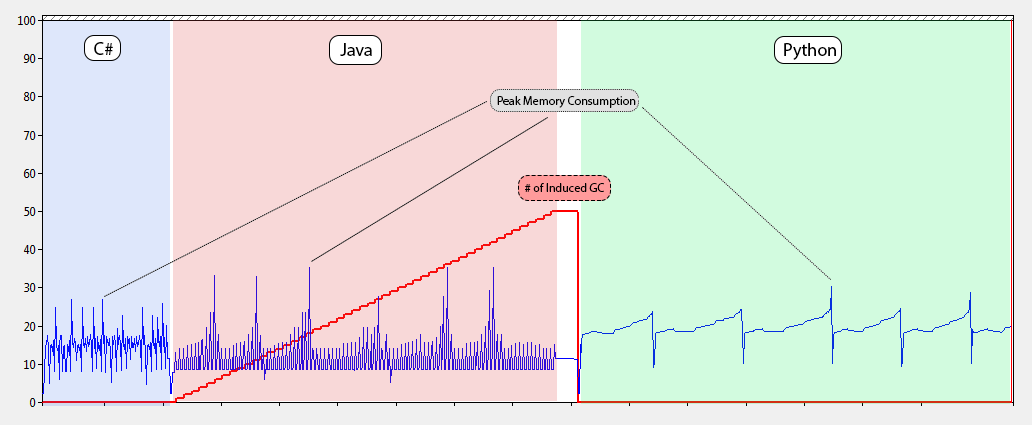
\includegraphics[width=1.0\textwidth]{chapters/media/mergesort_memory_1mil_all.png}
	\caption{Memory consumption over 100 test runs with one million elements for each language. Blue line represents memory consumption and red line represents the number of induced GC.}
	\label{fig:merge_sort_memory_all}
\end{figure}


Figure \ref{fig:merge_sort_memory_all} illustrates 100 runs with one million elements of the Merge Sort algorithm with each language run in .NET (all Python runs are not visible). It would appear that since the algorithm runs on the same input each run, one would expect a pattern to emerge. But due to restrictions in the Microsoft Performance Monitor it could only take one sample every second, and since C\# and Java ran faster than that, the plot is uneven. Therefore it is important to only consider the peak for each language. Several more runs were made in order to reduce the risk of data collection error, Figure \ref{fig:merge_sort_memory_all} is just an example run with all languages present to illustrate their differences (see Figure \ref{fig:merge_sort_memory} for  maximum values). The red line is the number of times the garbage collector was induced, note that Java forces this induction every other run.


\begin{figure}[h]
	\centering
	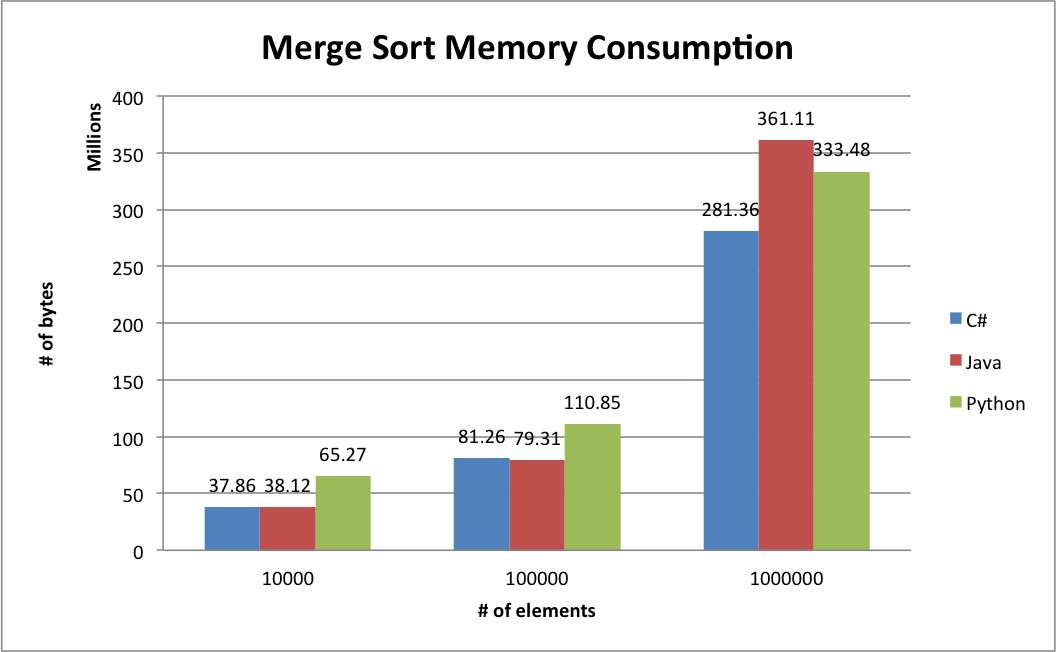
\includegraphics[width=1.0\textwidth]{chapters/media/merge_sort_memory.png}
	\caption{Comparison of the memory consumption between the three languages.}
	\label{fig:merge_sort_memory}
\end{figure}

The maximum memory consumption can be seen in Figure \ref{fig:merge_sort_memory}. Java consumed the most memory while C\# consumed the least.





























\chapter{Discussion}

%\chapter{References}


\appendix
\addappheadtotoc
\chapter{RDF}\label{appA}

\begin{figure}[ht]
\begin{center}
And here is a figure
\caption{\small{Several statements describing the same resource.}}\label{RDF_4}
\end{center}
\end{figure}

that we refer to here: \ref{RDF_4}



\bibliography{chapters/mybib}
\bibliographystyle{plain}

\end{document}
